\section{Lottery scheduling}
\emph{Lottery scheduling} es un algoritmo de planificación probabilístico para los procesos de un sistema operativo. A cada proceso se les asigna un número de billetes de lotería, y se elije un boleto al azar para seleccionar el siguiente proceso. La distribución de los billetes no tiene por qué ser uniforme, darle más billetes a un proceso le ofrece una oportunidad mayor de salir seleccionado.

\subsection{Implementación propuesta}
A la hora de implementar este algoritmo, recurrimos al \emph{paper} de Waldspurger y Weihl, \emph{Lottery scheduling: Flexible proportional - share resource management} el cual explica los detalles del algoritmo. 

En dicho \emph{paper}, además del sistema de tickets se propone un sistema de monedas o \emph{currencies} las cuales respaldan los \emph{tickets}. El sistema cuenta con una moneda base que respalda una serie de \emph{tickets} repartidos entre los usuarios que lanzan los procesos. A su vez, cada usuario emite una moneda para respaldar los \emph{tickets} que reciben sus procesos. Lo mismo sucede con los procesos y sus \emph{threads}. Como en el simulador provisto por la cátedra no existen los usuarios ni los \emph{threads}, implementamos únicamente el sistema de \emph{tickets} base.

A continuación explicaremos los pasos de nuestra implementación que utiliza los mismos métodos que la vista para \emph{Round Robin}.

\begin{itemize}
	\item El método \emph{load(pid)} se agrega a nuestro diccionario de tareas el nuevo \emph{pid} y se le da un \emph{ticket}.
	\item El método \emph{unblock(pid)} se la desmarca como bloqueada.
	\item El método \emph{tick(motivo)} se ejecuta por cada \emph{tick} del reloj de la máquina. El parámetro \textbf{motivo} indica lo que ocurrió con la tarea que ocupaba el procesador el ciclo de reloj anterior:
	
	\begin{itemize}
		\item Si el \textbf{motivo} es \emph{exit}: se saca la tarea de nuestro diccionario y se hace un nuevo sorteo.
		\item Si el \textbf{motivo} es \emph{block}: se la demarca como bloqueada y se la compensa con $\frac{quantum}{quantum - f}$ donde $f$ es la fracción de \emph{quantum} que utilizó.
		\item Si el \textbf{motivo} es \emph{tick}: si se termina el \emph{quantum} de esa tarea, se la desaloja y se realiza un sorteo. La nueva tarea elegida es puesta a trabajar y se le deja un solo \emph{ticket}. Si no hay más tareas o están todas bloqueadas, trabaja la \verb|idle_task|.
	\end{itemize}
\end{itemize}

\subsection{Diagrama de estados}
\begin{figure}[H]
\centering
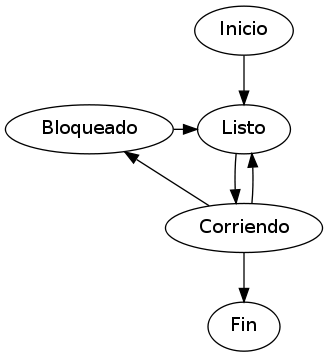
\includegraphics[scale=0.5]{estados.png}
\caption{El diagrama de estados es similar al del Round Robin.}
\end{figure}

\subsection{Análisis del algoritmo}
Para probar el algoritmo, le pasamos el siguiente lote:
\begin{verbatim}
	# lote_ej_8.tsk
	TaskIO 10 80
	*3 TaskCPU 60
	@10:
	TaskAlterno 10 20 10 20 10
	TaskAlterno 1 20 1 20 1 20
	TaskBatch 40 5
	@30:
	TaskCPU 50
	TaskBatch 40 5
\end{verbatim}

Con este lote lo que podemos observar es que las tareas que se bloquean (la 0, 4, 5, 6 y 8), no pasan mucho tiempo esperando el procesador, ya que son compensadas. Sin embargo, si miramos las tareas 1, 2 ó 7, vemos que pueden pasar varios turnos sin ocupar el procesador, ya tienen un solo ticket para el sorteo.

\begin{figure}[H]
\centering
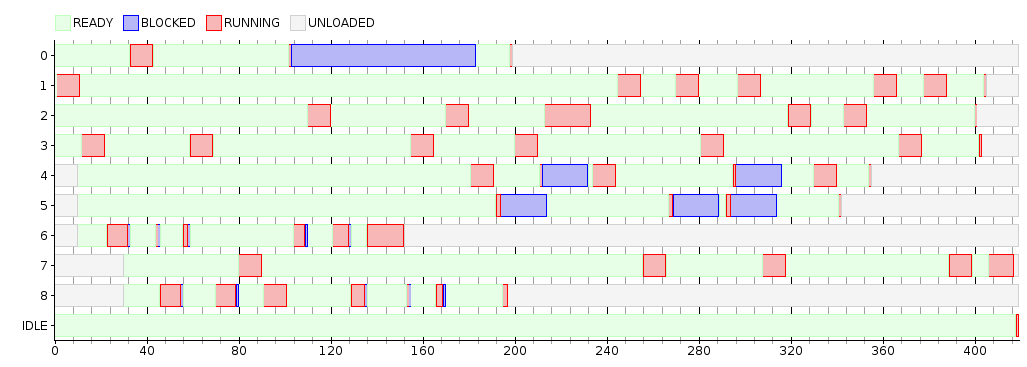
\includegraphics[scale=0.5]{./graficos/out_ej_8.png}
\caption{\emph{Lottery} - \emph{Quantum} 10, Semilla 1315772865, Lote con bloqueos.}
\end{figure} 

Las dos pruebas siguientes están hechas sobre el mismo lote, pero con diferente semilla y están para comprobar la naturaleza aleatoria del algoritmo.

\begin{figure}[H]
\centering
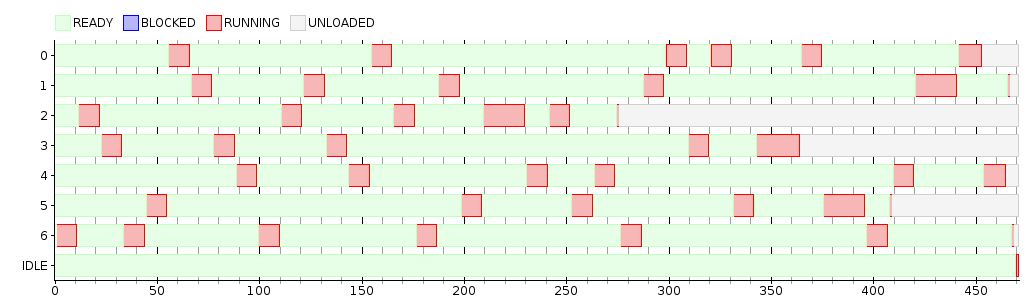
\includegraphics[scale=0.5]{./graficos/out_ej_8_2.png}
\caption{\emph{Lottery} - \emph{Quantum} 10, Semilla 1315772865, Lote sin bloqueos.}
\end{figure} 

\begin{figure}[H]
\centering
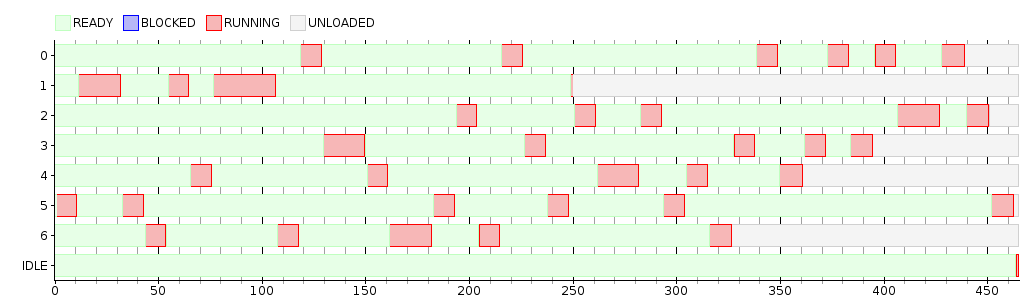
\includegraphics[scale=0.5]{./graficos/out_ej_8_3.png}
\caption{\emph{Lottery} - \emph{Quantum} 10, Semilla 1315793579, Lote sin bloqueos.}
\end{figure} 

